\documentclass[12pt]{article}

\usepackage{graphicx}
\usepackage{paralist}
\usepackage{amsfonts}
\usepackage{amsmath}
\usepackage{hhline}
\usepackage{booktabs}
\usepackage{multirow}
\usepackage{multicol}
\usepackage{url}
\usepackage{pdfpages}

\oddsidemargin -10mm
\evensidemargin -10mm
\textwidth 160mm
\textheight 200mm
\renewcommand\baselinestretch{1.0}

\pagestyle {plain}
\pagenumbering{arabic}

\newcounter{stepnum}

%% Comments

\usepackage{color}

\newif\ifcomments\commentstrue

\ifcomments
\newcommand{\authornote}[3]{\textcolor{#1}{[#3 ---#2]}}
\newcommand{\todo}[1]{\textcolor{red}{[TODO: #1]}}
\else
\newcommand{\authornote}[3]{}
\newcommand{\todo}[1]{}
\fi

\newcommand{\wss}[1]{\authornote{blue}{SS}{#1}}

\title{Assignment 4, Design Specification}
\author{SFWRENG 2AA4}

\begin{document}

\maketitle
This Module Interface Specification (MIS) document contains the modules necessary to implement the model and the view of the game \textit{2048}. At the start of the game, the player will see a 4x4 board containing 16 cells. Two random cells will contain either two \texttt{2} tiles, or one \texttt{2} tile and one \texttt{4} tile. The player can then move the tiles either up, down, left, or right, and the tiles slide over in that direction as far as they can go, unless they are blocked by the edge of the board, or another tile. If the tiles that slide together are the same, then they combine to create a single tile whose value is two times its original value. Therefore, all cells are either empty, or contain a tile whose value is $2^n$, where $n$ is a natural number not including $0$. After that, a random empty cell will be replaced by a \texttt{2} tile. For this implementation, the empty cells will be represented by a \texttt{0} tile. A visualization of the game board and an example of a move \texttt{right} is shown below:

\begin{center}
  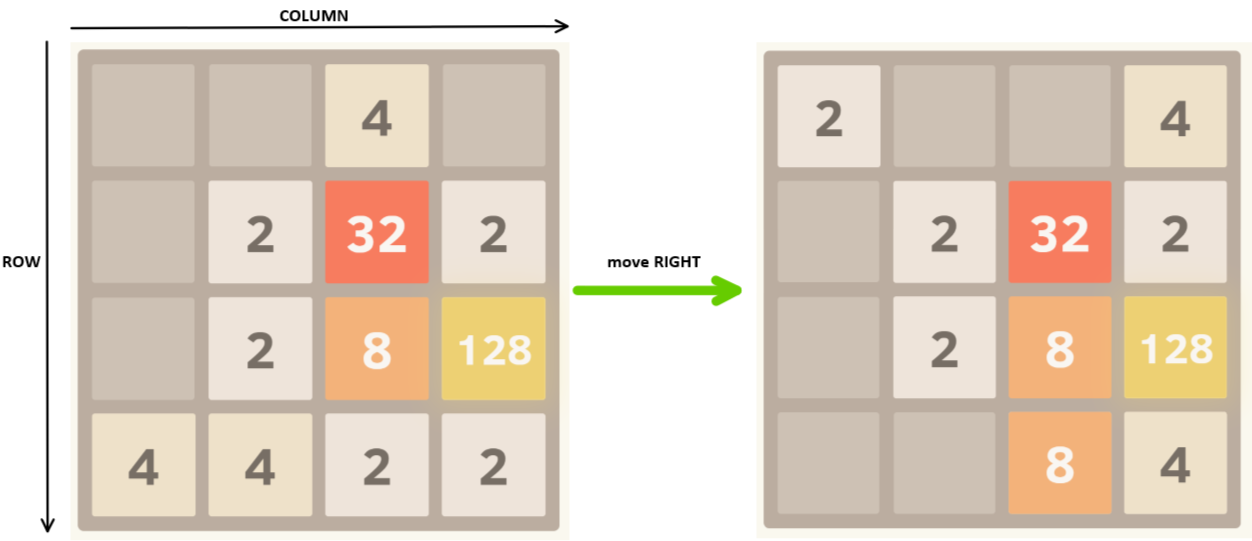
\includegraphics[width=0.9\textwidth]{moveright.PNG}
\end{center}

\newpage

\section{Overview of the design}

This design applies Model View Controller (MVC) design pattern, where \textit{BoardT} is the model module and \textit{View} is the view module. The module \textit{BoardT} stores the state of the game board and the status of the game, while the view module \textit{View} displays the current state of the game board and the overall game using text-based (ASCII) graphics. There is no controller module in this implementation.

\newpage

\subsection*{Likely Changes my design considers:}

\begin{itemize}
  \item The interface that enables the player to play the game.
  \item The peripheral devices used to take input from the player.
  \item The data structure used for storing the board.
  \item The interface that provides a visual display of the game to the player.
\end{itemize}

\newpage

\section* {Board ADT Module}

\subsection*{Template Module}

BoardT

\subsection* {Uses}

None

\subsection* {Syntax}

\subsubsection* {Exported Types}

None

\subsubsection* {Exported Constant}

size = 4 \quad // Size of the board 4 x 4

\subsubsection* {Exported Access Programs}

\begin{tabular}{| l | l | l | l |}
\hline
\textbf{Routine name} & \textbf{In} & \textbf{Out} & \textbf{Exceptions}\\
\hline
BoardT & ~ & BoardT & \\
\hline
getBoard & ~ & seq of (seq of $\mathbb{N}$) & \\
\hline
getScore & ~ & $\mathbb{N}$ & \\
\hline
getHighScore & ~ & $\mathbb{N}$ & \\
\hline
emptyCells & ~ & set of (seq of $\mathbb{N}$) & \\
\hline
isGameWon & ~ & $\mathbb{B}$ & \\
\hline
isGameLost & ~ & $\mathbb{B}$ & \\
\hline
setBoard & seq of (seq of $\mathbb{N}$) & ~ & IllegalArgumentException\\
\hline
resetBoard  & ~ &  ~     & \\
\hline
isValidMoveRight  & ~ &  $\mathbb{B}$   & \\
\hline
isValidMoveLeft  &  ~  &  $\mathbb{B}$   & \\
\hline
isValidMoveUp  &  ~  &  $\mathbb{B}$   & \\
\hline
isValidMoveDown  &  ~  & $\mathbb{B}$ & \\
\hline
moveRight  & ~  &  ~     & \\
\hline
moveLeft  &  ~ &  ~     & \\
\hline
moveUp  &  ~  &  ~     & \\
\hline
moveDown  &  ~  &  ~     & \\
\hline
\end{tabular}

\subsection* {Semantics}

\subsubsection* {State Variables}

board: sequence [size, size] of $\mathbb{N}$ \\
score: $\mathbb{N}$ \\
highscore: $\mathbb{N}$ \\
empty: set of (sequence of $\mathbb{N}$) \\
win: $\mathbb{B}$ \\
lose: $\mathbb{B}$

\subsubsection* {State Invariant}

$0 \le |empty| \le 14$\\
$0 \le score \le highscore$

\subsubsection* {Assumptions}

\begin{itemize}
  \item The constructor BoardT is called for each object instance before any other access routine 
  is called for that object. 
  \item Assume there is a random function that generates a random value between 0 and 1.
  \item \textit{highscore} is a static variable.
  \item The seq of (seq of $\mathbb{N}$) provided as input for the \textit{setBoard} method will consist of correct numbers. This means that the numbers will be either $0$ to represent an empty cell, or $2^n$, where $n \ne 0$.
  \item The set of (sequence of $\mathbb{N}$) used to represent the state variable \textit{empty} will contain the coordinates for the empty cells of the game board. The sequence of $\mathbb{N}$ will only contain two numbers to represent the row and column of an empty cell. For example, \textit{empty} will be a set of $[row, column]$.
\end{itemize}

\subsubsection* {Access Routine Semantics}

BoardT():
\begin{itemize}
\item transition: \\
      board $:=$ 
      $\langle \begin{array}{c}
      \langle 0, 0, 0, 0 \rangle\\
      \langle 0, 0, 0, 0 \rangle\\
      \langle 0, 0, 0, 0 \rangle\\
      \langle 0, 0, 0, 0 \rangle\\
      \end{array} \rangle$ \\ 
      where two random empty cells are replaced with two \texttt{2} tiles or one \texttt{2} tile and one \texttt{4} tile.

      score, win, lose $=$ 0, False, False\\
      empty $:= \forall i, j : [0...size-1] | (board[i][j] = 0 \Rightarrow empty \cup \{\langle i, j \rangle\}$ $|$ $True \Rightarrow empty - \{\langle i, j \rangle\}$)
\item output: $out := \mathit{self}$
\item exception: None
\end{itemize}

\noindent getBoard():
\begin{itemize}
\item output: $out :=$ board
\item exception: None
\end{itemize}

\noindent getScore():
\begin{itemize}
\item output: $out :=$ score
\item exception: None
\end{itemize}

\noindent getHighScore():
\begin{itemize}
\item output: $out :=$ highscore
\item exception: None
\end{itemize}

\noindent emptyCells():
\begin{itemize}
\item output: $out :=$ empty
\item exception: None
\end{itemize}

\noindent isGameWon():
\begin{itemize}
\item output: $out :=$ win
\item exception: None
\end{itemize}

\noindent isGameLost():
\begin{itemize}
\item output: $out :=$ lose
\item exception: None
\end{itemize}

\noindent setBoard($b$):
\begin{itemize}
  \item transition: board $:= b$ 
  \item output: None
  \item exception: $exc :=$ (($\neg$ ($|b| = 4$) 
  $\Rightarrow$ IllegalArgumentException) $|$ 
  ($\forall(i : [0...size-1]$ $|$ $\neg (|b[i]| = 4) \Rightarrow$ IllegalArgumentException)))
\end{itemize}

\noindent resetBoard():
\begin{itemize}
\item transition:\\
      board $:=$ 
      $\langle \begin{array}{c}
      \langle 0, 0, 0, 0 \rangle\\
      \langle 0, 0, 0, 0 \rangle\\
      \langle 0, 0, 0, 0 \rangle\\
      \langle 0, 0, 0, 0 \rangle\\
      \end{array} \rangle$ \\ 
      where two random empty cells are replaced with two \texttt{2} tiles or one \texttt{2} tile and one \texttt{4} tile.

      score, win, lose $=$ 0, False, False\\
      empty $:= \forall i, j : [0...size-1] | (board[i][j] = 0 \Rightarrow empty \cup \{\langle i, j \rangle\}$ $|$ $True \Rightarrow empty - \{\langle i, j \rangle\}$)
\item output: None
\item exception: None
\end{itemize}

\noindent isValidMoveRight():
\begin{itemize}
\item output: $\forall i : [0...size-1]$ $(\forall j : [0...size-2]$ $|$ $(board[i][j] \ne 0 \land board[i][j+1]=0 \Rightarrow True$ $|$ $board[i][j] = board[i][j+1] \land board[i][j], board[i][j+1] \ne 0 \Rightarrow True$ $|$ $True \Rightarrow False))$
\item exception: None
\end{itemize}

\noindent isValidMoveLeft():
\begin{itemize}
\item output: $\forall i : [0...size-1]$ $(\forall j : [size-1...1]$ $|$ $(board[i][j] \ne 0 \land board[i][j-1]=0 \Rightarrow True$ $|$ $board[i][j] = board[i][j-1] \land board[i][j], board[i][j-1] \ne 0 \Rightarrow True$ $|$ $True \Rightarrow False))$
\item exception: None
\end{itemize}

\noindent isValidMoveUp():
\begin{itemize}
\item output: $\forall i : [size-1...1]$ $(\forall j : [0...size-1]$ $|$ $(board[i][j] \ne 0 \land board[i-1][j]=0 \Rightarrow True$ $|$ $board[i][j] = board[i-1][j] \land board[i][j], board[i-1][j] \ne 0 \Rightarrow True$ $|$ $True \Rightarrow False))$
\item exception: None
\end{itemize}

\noindent isValidMoveDown():
\begin{itemize}
\item output: $\forall i : [0...size-2]$ $(\forall j : [0...size-1]$ $|$ $(board[i][j] \ne 0 \land board[i+1][j]=0 \Rightarrow True$ $|$ $board[i][j] = board[i+1][j] \land board[i][j], board[i+1][j] \ne 0 \Rightarrow True$ $|$ $True \Rightarrow False))$
\item exception: None
\end{itemize}

\noindent moveRight():
\begin{itemize}
\item transition:\\ 
board $:=$ $\forall i : [0...size-1]$ $(\forall j : [0...size-2]$ $|$
\begin{table}[hbt!]
\centering
\begin{tabular}{|l|l|l|}
\cline{3-3}
\multicolumn{1}{l}{} &  & transition \\
\hline
\multicolumn{2}{|l|}{$board[i][j] \ne 0 \land board[i][j+1] = 0$} & board $:=$ shiftRight(i, j, board)\\
\hline
\shortstack{$(board[i][j], board[i][j+1] \ne 0$ \\$\land board[i][j] = board[i][j+1]$} & \shortstack{$2\times board[i][j] = 2048 \land$ \\ $\neg$(score $+ \: 2\times board[i][j] > $ highscore) } & \shortstack{board $:=$ combineRight(i, j, board)\\ score $:=$ score $+\: 2\times board[i][j]$\\ win $:=$ True}\\
\cline{2-3}
 & \shortstack{$2\times board[i][j] \ne 2048 \land$ \\ (score $+ \: 2\times board[i][j] > $ highscore) } & \shortstack{board $:=$ combineRight(i, j, board)\\ score $:=$ score $+\: 2\times board[i][j]$\\ highscore $:=$ score $+\: 2\times board[i][j]$}\\
\cline{2-3}
  & \shortstack{$2\times board[i][j] = 2048 \land$ \\ (score $+ \: 2\times board[i][j] > $ highscore) }  & \shortstack{board $:=$ combineRight(i, j, board)\\ score $:=$ score $+\: 2\times board[i][j]$\\ highscore $:=$ score $+\: 2\times board[i][j]$\\ win $:=$ True}\\
\cline{2-3}
  & True & \shortstack{board $:=$ combineRight(i, j, board)\\ score $:=$ score $+\: 2\times board[i][j]$}\\
\hline
\end{tabular}
\end{table}
\\
) // \textit{And also replaces one random empty cell (if it exists) with a \texttt{2} tile.}\\
lose $:= \neg$ (isValidMoveRight() $\lor$ isValidMoveLeft() $\lor$ isValidMoveUp $\lor$ isValidMoveDown()) $\Rightarrow True$\\
empty $:= \forall i, j : [0...size-1] | (board[i][j] = 0 \Rightarrow empty \cup \{\langle i, j \rangle\}$ $|$ $True \Rightarrow empty - \{\langle i, j \rangle\}$)
\item output: None
\item exception: None
\end{itemize}

\newpage

\noindent moveLeft():
\begin{itemize}
\item transition:\\ 
board $:=$ $\forall i : [0...size-1]$ $(\forall j : [size-1...1]$ $|$
\begin{table}[hbt!]
\centering
\begin{tabular}{|l|l|l|}
\cline{3-3}
\multicolumn{1}{l}{} &  & transition \\
\hline
\multicolumn{2}{|l|}{$board[i][j] \ne 0 \land board[i][j-1] = 0$} & board $:=$ shiftLeft(i, j, board)\\
\hline
\shortstack{$(board[i][j], board[i][j-1] \ne 0$ \\$\land board[i][j] = board[i][j-1]$} & \shortstack{$2\times board[i][j] = 2048 \land$ \\ $\neg$(score $+ \: 2\times board[i][j] > $ highscore) } & \shortstack{board $:=$ combineLeft(i, j, board)\\ score $:=$ score $+\: 2\times board[i][j]$\\ win $:=$ True}\\
\cline{2-3}
 & \shortstack{$2\times board[i][j] \ne 2048 \land$ \\ (score $+ \: 2\times board[i][j] > $ highscore) } & \shortstack{board $:=$ combineLeft(i, j, board)\\ score $:=$ score $+\: 2\times board[i][j]$\\ highscore $:=$ score $+\: 2\times board[i][j]$}\\
\cline{2-3}
  & \shortstack{$2\times board[i][j] = 2048 \land$ \\ (score $+ \: 2\times board[i][j] > $ highscore) }  & \shortstack{board $:=$ combineLeft(i, j, board)\\ score $:=$ score $+\: 2\times board[i][j]$\\ highscore $:=$ score $+\: 2\times board[i][j]$\\ win $:=$ True}\\
\cline{2-3}
  & True & \shortstack{board $:=$ combineLeft(i, j, board)\\ score $:=$ score $+\: 2\times board[i][j]$}\\
\hline
\end{tabular}
\end{table}
\\
) // \textit{And also replaces one random empty cell (if it exists) with a \texttt{2} tile.}\\
lose $:= \neg$ (isValidMoveRight() $\lor$ isValidMoveLeft() $\lor$ isValidMoveUp $\lor$ isValidMoveDown()) $\Rightarrow True$\\
empty $:= \forall i, j : [0...size-1] | (board[i][j] = 0 \Rightarrow empty \cup \{\langle i, j \rangle\}$ $|$ $True \Rightarrow empty - \{\langle i, j \rangle\}$)
\item output: None
\item exception: None
\end{itemize}

\newpage

\noindent moveUp():
\begin{itemize}
\item transition:\\ 
board $:=$ $\forall i : [size-1...1]$ $(\forall j : [0...size-1]$ $|$
\begin{table}[hbt!]
\centering
\begin{tabular}{|l|l|l|}
\cline{3-3}
\multicolumn{1}{l}{} &  & transition \\
\hline
\multicolumn{2}{|l|}{$board[i][j] \ne 0 \land board[i-1][j] = 0$} & board $:=$ shiftUp(i, j, board)\\
\hline
\shortstack{$(board[i][j], board[i-1][j] \ne 0$ \\$\land board[i][j] = board[i-1][j]$} & \shortstack{$2\times board[i][j] = 2048 \land$ \\ $\neg$(score $+ \: 2\times board[i][j] > $ highscore) } & \shortstack{board $:=$ combineUp(i, j, board)\\ score $:=$ score $+\: 2\times board[i][j]$\\ win $:=$ True}\\
\cline{2-3}
 & \shortstack{$2\times board[i][j] \ne 2048 \land$ \\ (score $+ \: 2\times board[i][j] > $ highscore) } & \shortstack{board $:=$ combineUp(i, j, board)\\ score $:=$ score $+\: 2\times board[i][j]$\\ highscore $:=$ score $+\: 2\times board[i][j]$}\\
\cline{2-3}
  & \shortstack{$2\times board[i][j] = 2048 \land$ \\ (score $+ \: 2\times board[i][j] > $ highscore) }  & \shortstack{board $:=$ combineUp(i, j, board)\\ score $:=$ score $+\: 2\times board[i][j]$\\ highscore $:=$ score $+\: 2\times board[i][j]$\\ win $:=$ True}\\
\cline{2-3}
  & True & \shortstack{board $:=$ combineUp(i, j, board)\\ score $:=$ score $+\: 2\times board[i][j]$}\\
\hline
\end{tabular}
\end{table}
\\
) // \textit{And also replaces one random empty cell (if it exists) with a \texttt{2} tile.}\\
lose $:= \neg$ (isValidMoveRight() $\lor$ isValidMoveLeft() $\lor$ isValidMoveUp $\lor$ isValidMoveDown()) $\Rightarrow True$\\
empty $:= \forall i, j : [0...size-1] | (board[i][j] = 0 \Rightarrow empty \cup \{\langle i, j \rangle\}$ $|$ $True \Rightarrow empty - \{\langle i, j \rangle\}$)
\item output: None
\item exception: None
\end{itemize}

\newpage

\noindent moveDown():
\begin{itemize}
\item transition:\\ 
board $:=$ $\forall i : [0...size-2]$ $(\forall j : [0...size-1]$ $|$
\begin{table}[hbt!]
\centering
\begin{tabular}{|l|l|l|}
\cline{3-3}
\multicolumn{1}{l}{} &  & transition \\
\hline
\multicolumn{2}{|l|}{$board[i][j] \ne 0 \land board[i+1][j] = 0$} & board $:=$ shiftDown(i, j, board)\\
\hline
\shortstack{$(board[i][j], board[i+1][j] \ne 0$ \\$\land board[i][j] = board[i+1][j]$} & \shortstack{$2\times board[i][j] = 2048 \land$ \\ $\neg$(score $+ \: 2\times board[i][j] > $ highscore) } & \shortstack{board $:=$ combineDown(i, j, board)\\ score $:=$ score $+\: 2\times board[i][j]$\\ win $:=$ True}\\
\cline{2-3}
 & \shortstack{$2\times board[i][j] \ne 2048 \land$ \\ (score $+ \: 2\times board[i][j] > $ highscore) } & \shortstack{board $:=$ combineDown(i, j, board)\\ score $:=$ score $+\: 2\times board[i][j]$\\ highscore $:=$ score $+\: 2\times board[i][j]$}\\
\cline{2-3}
  & \shortstack{$2\times board[i][j] = 2048 \land$ \\ (score $+ \: 2\times board[i][j] > $ highscore) }  & \shortstack{board $:=$ combineDown(i, j, board)\\ score $:=$ score $+\: 2\times board[i][j]$\\ highscore $:=$ score $+\: 2\times board[i][j]$\\ win $:=$ True}\\
\cline{2-3}
  & True & \shortstack{board $:=$ combineDown(i, j, board)\\ score $:=$ score $+\: 2\times board[i][j]$}\\
\hline
\end{tabular}
\end{table}
\\
) // \textit{And also replaces one random empty cell (if it exists) with a \texttt{2} tile.}\\
lose $:= \neg$ (isValidMoveRight() $\lor$ isValidMoveLeft() $\lor$ isValidMoveUp $\lor$ isValidMoveDown()) $\Rightarrow True$\\
empty $:= \forall i, j : [0...size-1] | (board[i][j] = 0 \Rightarrow empty \cup \{\langle i, j \rangle\}$ $|$ $True \Rightarrow empty - \{\langle i, j \rangle\}$)
\item output: None
\item exception: None
\end{itemize}

\subsubsection* {Local Functions}

shiftRight: $\mathbb{N} \times \mathbb{N} \times$ seq of (seq of $\mathbb{N}$) $\rightarrow$ seq of (seq of $\mathbb{N}$) 

\medskip

\noindent shiftRight($i, j, board$) $\equiv$ $\forall x : [j+1...0]$ $|$ $(x = 0 \Rightarrow board[i][x] = 0$ $|$ $True \Rightarrow board[i][x] = board[i][x-1])$

\bigskip
\bigskip

\noindent combineRight: $\mathbb{N} \times \mathbb{N} \times$ seq of (seq of $\mathbb{N}$) $\rightarrow$ seq of (seq of $\mathbb{N}$)

\medskip

\noindent combineRight($i, j, board$) $\equiv$ $\forall x : [j+1...0]$ $|$ $(x = j+1 \Rightarrow board[i][x] = 2 \times board[i][x]$ $|$ $x = 0 \Rightarrow board[i][x] = 0$ $|$ $True \Rightarrow board[i][x] = board[i][x-1])$

\bigskip
\bigskip

\noindent shiftLeft: $\mathbb{N} \times \mathbb{N} \times$ seq of (seq of $\mathbb{N}$) $\rightarrow$ seq of (seq of $\mathbb{N}$) 

\medskip

\noindent shiftLeft($i, j, board$) $\equiv$ $\forall x : [j-1...size-1]$ $|$ $(x = 0 \Rightarrow board[i][x] = 0$ $|$ $True \Rightarrow board[i][x] = board[i][x+1])$

\bigskip
\bigskip

\noindent combineLeft: $\mathbb{N} \times \mathbb{N} \times$ seq of (seq of $\mathbb{N}$) $\rightarrow$ seq of (seq of $\mathbb{N}$)

\medskip

\noindent combineLeft($i, j, board$) $\equiv$ $\forall x : [j-1...size-1]$ $|$ $(x = j-1 \Rightarrow board[i][x] = 2 \times board[i][x]$ $|$ $x = size-1 \Rightarrow board[i][x] = 0$ $|$ $True \Rightarrow board[i][x] = board[i][x+1])$

\bigskip
\bigskip

\noindent shiftUp: $\mathbb{N} \times \mathbb{N} \times$ seq of (seq of $\mathbb{N}$) $\rightarrow$ seq of (seq of $\mathbb{N}$) 

\medskip

\noindent shiftUp($i, j, board$) $\equiv$ $\forall x : [i-1...size-1]$ $|$ $(x = size-1 \Rightarrow board[x][j] = 0$ $|$ $True \Rightarrow board[x][j] = board[x+1][j])$

\bigskip
\bigskip

\noindent combineUp: $\mathbb{N} \times \mathbb{N} \times$ seq of (seq of $\mathbb{N}$) $\rightarrow$ seq of (seq of $\mathbb{N}$)

\medskip

\noindent combineUp($i, j, board$) $\equiv$ $\forall x : [i-1...size-1]$ $|$ $(x = i-1 \Rightarrow board[x][j] = 2 \times board[x][j]$ $|$ $x = size-1 \Rightarrow board[x][j] = 0$ $|$ $True \Rightarrow board[x][j] = board[x+1][j])$

\bigskip
\bigskip

\noindent shiftDown: $\mathbb{N} \times \mathbb{N} \times$ seq of (seq of $\mathbb{N}$) $\rightarrow$ seq of (seq of $\mathbb{N}$) 

\medskip

\noindent shiftDown($i, j, board$) $\equiv$ $\forall x : [i+1...0]$ $|$ $(x = 0 \Rightarrow board[x][j] = 0$ $|$ $True \Rightarrow board[x][j] = board[x-1][j])$

\bigskip
\bigskip

\noindent combineDown: $\mathbb{N} \times \mathbb{N} \times$ seq of (seq of $\mathbb{N}$) $\rightarrow$ seq of (seq of $\mathbb{N}$)

\medskip

\noindent combineDown($i, j, board$) $\equiv$ $\forall x : [i+1...0]$ $|$ $(x = i+1 \Rightarrow board[x][j] = 2 \times board[x][j]$ $|$ $x = 0 \Rightarrow board[x][j] = 0$ $|$ $True \Rightarrow board[x][j] = board[x-1][j])$

\bigskip
\bigskip


\newpage

\section* {View Module}

\subsection* {Module}

View

\subsection* {Uses}

BoardT

\subsection* {Syntax}

\subsubsection* {Exported Types}

None

\subsubsection* {Exported Constants}

None

\subsubsection* {Exported Access Programs}

\begin{tabular}{| l | l | l | p{6cm} |}
\hline
\textbf{Routine name} & \textbf{In} & \textbf{Out} & \textbf{Exceptions}\\
\hline
printWelcomeMessage & ~ & ~ &  \\
\hline
printBoard & BoardT & ~ & \\
\hline
printMovePrompt & ~ & ~ & \\
\hline
printScore & BoardT & ~ & \\
\hline
printHighScore & BoardT & ~ & \\
\hline
printLosingMessage & ~ & ~ & \\
\hline
printWinningMessage & ~ & ~ & \\
\hline
printFarewellMessage & ~ & ~ & \\
\hline
\end{tabular}

\subsection* {Semantics}

\subsubsection* {Environment Variables}

terminal: displays the game, messages, and prompts to the player

\subsubsection* {State Variables}

None

\subsubsection* {State Invariant}

None

\subsubsection* {Access Routine Semantics}

\noindent printWelcomeMessage():
\begin{itemize}
  \item transition: terminal $:=$ Displays a welcome message when the player begins the game for the first time.
\end{itemize}

\noindent printBoard():
\begin{itemize}
\item transition: terminal $:=$ Displays the game board. The cells can be accessed by using the $getBoard$ method from $BoardT$. The board is displayed as a 4x4 matrix, so each row of cells is on a separate line. The board[x][y] is displayed so that x increases as you go right across the screen, and y increases as you go down the screen.
\end{itemize}

\noindent printMovePrompt():
\begin{itemize}
\item transition: terminal $:=$ Displays a prompt asking the player to select which direction they want to move the tiles.
\end{itemize}

\noindent printScore($b$):
\begin{itemize}
\item transition: terminal $:=$ Displays the current score of the game, which can be accessed by using the $getScore$ method from $BoardT$.
\end{itemize}

\noindent printHighScore($b$):
\begin{itemize}
\item transition: terminal $:=$ Displays the best/highest score of the game, which can be accessed by using the $getHighScore$ method from $BoardT$.
\end{itemize}

\noindent printLosingMessage():
\begin{itemize}
\item transition: terminal $:=$ Displays a message telling the player they lost, then displays a prompt asking the player if they would like to try again or exit the game.
\end{itemize}

\noindent printWinningMessage():
\begin{itemize}
\item transition: terminal $:=$ Displays a message telling the player they won, then displays a prompt asking the player if they would like to continue the current game, start a new game, or exit the game.
\end{itemize}

\noindent printFarewellMessage():
\begin{itemize}
\item transition: terminal $:=$ Displays a farewell message after the player decides to exit the game.
\end{itemize}

\newpage

\section*{Critique of Design}

\begin{itemize}
  \item The BoardT module is an abstract data type instead of an abstract object. This is so multiple instances can be created at a time, and therefore, multiple games can be played. Player A does not have to reset their game if Player B wants to start their own game. Also, this makes it easier to implement the $resetBoard()$ method for if the player would like to reset the game.
  \item The View module is implemented as a library of methods. This is because the View module only contains methods that print out different messages along with the current state of the board. That means you don't need to create an instance of a View to use the methods, you can just call them when needed.
  \item The $resetBoard()$ method from the BoardT module is not essential, since instead of resetting the board/game, you can also just create a new instance of the board.
  \item The $emptyCells()$ method from the BoardT module is also not essential. You can figure out which cells are empty by looking at the board, which you can see by using the $getBoard()$ method.
  \item The BoardT module is not minimal. This is because $resetBoard()$, $moveRight()$, $moveLeft()$, $moveUp()$, and $moveDown()$ all make changes to multiple state variables at once. For example, $moveRight()$ changes the state of the board, the score, the empty cells, and possibly even win, lose, and the highscore.
  \item The $setBoard()$ method is mostly for the programmer and can be used for testing purposes. This way the programmer knows what the board looks like, and it is not randomly generated. A randomly generated board makes it difficult to use automated testing.
  \item My implementation of the $moveRight()$, $moveLeft()$, $moveUp()$, and $moveDown()$ methods were not very abstract or general, since they only account for a 4x4 game board.
  \item Applying the MVC (or MV in this case) design pattern promotes the maintainability of the interface. It also applies separation of concerns since the model module and view module contain methods mostly independent of each other; the model module handles storing the state and status of the game, while the view module displays the current status of the game.
  \item The MVC design pattern promotes high cohesion since BoardT and View are closely related. The methods of View are based entirely on the model of the game implemented in BoardT.
  \item The MVC design pattern also promotes low coupling since the model and view modules are almost entirely independent of each other. This way, changing one module will not greatly affect the other module.
  
\end{itemize}

\bigskip

\section*{Answers to Questions}

\noindent Q1: Draw a UML diagram for the modules in A3.

\noindent Q2: Draw a control flow graph for the convex hull algorithm.

\noindent The diagrams for these questions are below:

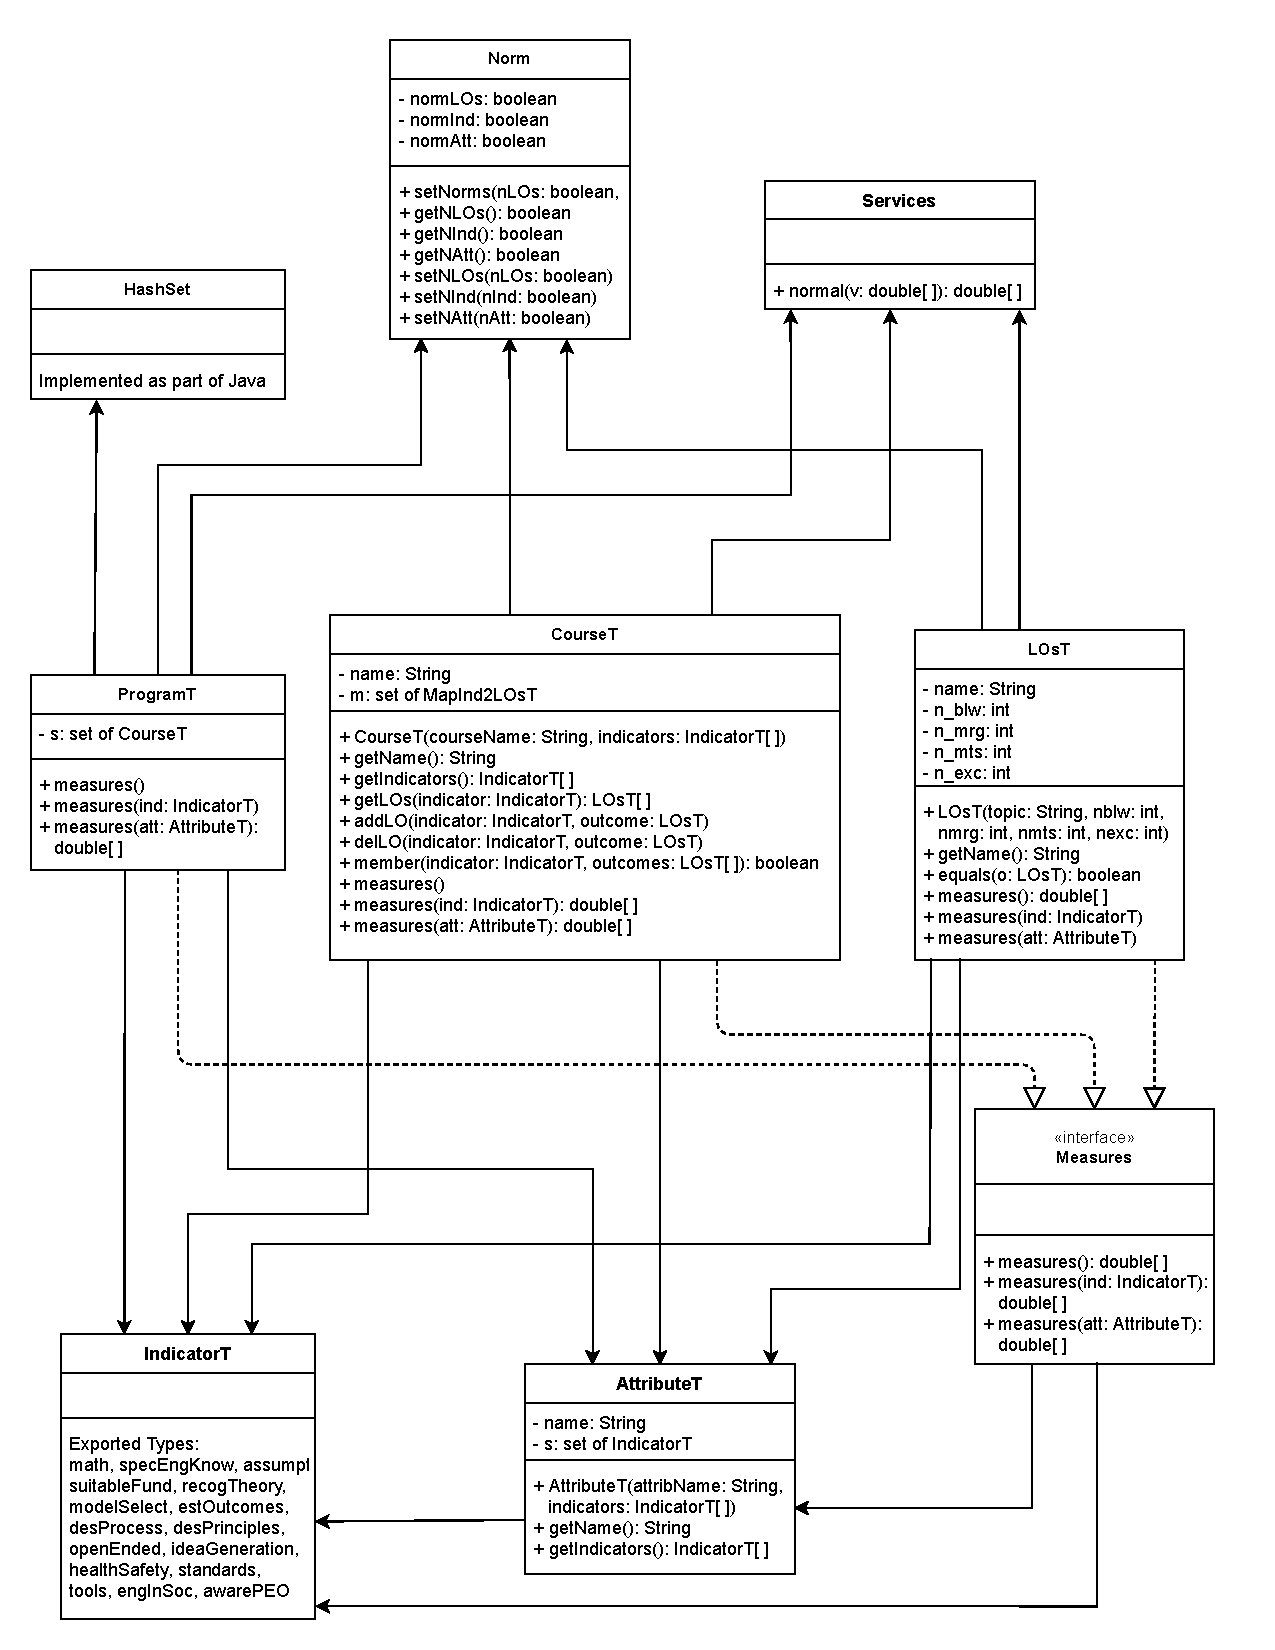
\includepdf[pages=-]{A3UML.pdf}
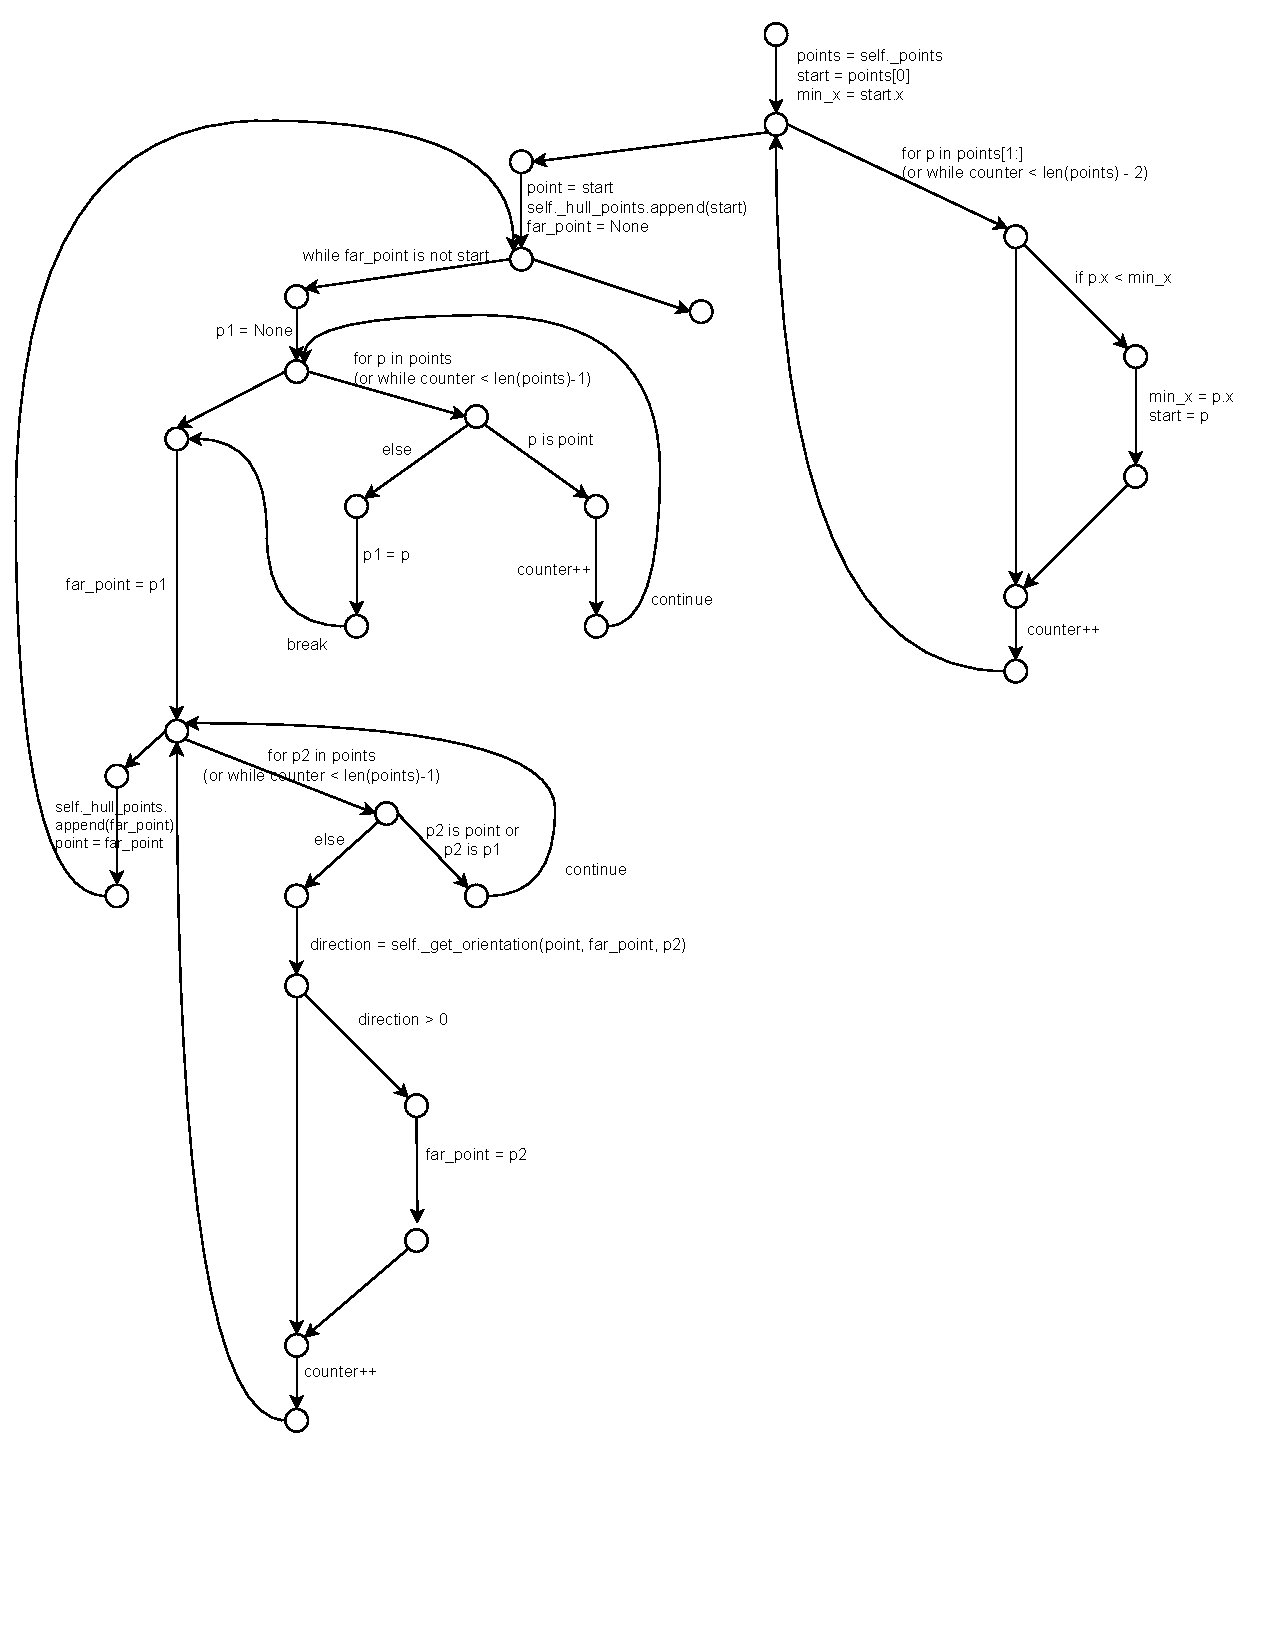
\includepdf[pages=-]{ControlFlow.pdf}

\end {document}